\section{Throughput Analysis}
\label{sec:throughput}

% GUIDANCE: This is the mathematical core of the paper. Derive the throughput
% scaling law and optimal satellite distribution from the relay tradeoff
% (ring count vs route count). Include both analytical derivations and
% simulation/spreadsheet validation.


\subsection{Link Budget Model}
\label{sec:link-budget}

% TODO: Write prose introducing the inverse-square model.

The capacity of a single free-space optical link at distance $d$ is modelled by the
inverse-square law:
%
\begin{equation}\label{eq:link-capacity}
  C(d) \;=\; f \, C_0 \left(\frac{d_0}{d}\right)^{\!2}
\end{equation}
%
where $C_0 = 100\Gbps$ is the baseline capacity at reference distance
$d_0 = 3{,}000\km$ (consistent with NASA TBIRD-class demonstrations), and $f$ is a
technology improvement factor reflecting advances in laser power, receiver sensitivity,
and modulation efficiency. We define the constant
%
\begin{equation}\label{eq:K}
  K \;=\; f \, C_0 \, d_0^2
\end{equation}
%
With $f = 1$ (no improvement), $K = 9 \times 10^{8}\;\text{Gbps}\cdot\text{km}^2$.
% NOTE: the marslink.py analysis uses f=10, K=9e12 Mbps*km^2. Decide which
% baseline to present as default and discuss sensitivity to f in a subsection.


\subsection{Constellation Geometry}
\label{sec:geometry}

% TODO: Write prose describing the relay ring layout.

Consider $R$ relay rings placed on concentric heliocentric circular orbits between
Earth's orbit (radius $\rE \approx 150\;\text{Mkm}$) and Mars' orbit
(radius $\rM \approx 228\;\text{Mkm}$ average, $249\;\text{Mkm}$ at apoapsis). Each ring contains $N$ satellites
evenly spaced around its circumference. The total relay satellite count is $S = N \times R$.
Each satellite carries exactly two laser terminals --- one pointing radially inward to the
adjacent inner ring, one pointing radially outward to the adjacent outer ring. There are
no circumferential (intra-ring) links. This creates $N$ parallel \emph{routes}, each a
radial chain hopping from ring~1 (nearest Earth) through to ring~$R$ (nearest Mars).

Ring~$i$ ($i = 1, \ldots, R$) sits at heliocentric radius
%
\begin{equation}
  r_i \;=\; \rE + i \,\frac{\Dem}{R+1}
\end{equation}
%
where $\Dem = \rM - \rE$. Using average orbital radii, $\Dem \approx 78\;\text{Mkm}$;
at Mars apoapsis, $\Dem \approx 99\;\text{Mkm}$. The inter-ring radial gap is
%
\begin{equation}\label{eq:d-radial}
  d_{\text{radial}} \;=\; \frac{\Dem}{R+1}
\end{equation}
%
and the arc spacing between adjacent satellites on ring~$i$ is $2\pi r_i / N$.

% NOTE: Earth and Mars co-orbit rings are separate systems that connect the
% relay to the ground. They are not part of this analysis.


\subsection{Worst-Case Inter-Ring Link Distance}
\label{sec:worst-case}

A satellite on ring~$i$ connects to the \emph{nearest} satellite on ring~$i+1$. In the
worst case, the nearest neighbor is offset by half the arc spacing on ring~$i+1$. The
worst-case link distance between adjacent rings is therefore
%
\begin{equation}\label{eq:d-worst}
  d_{\text{worst}} \;=\; \sqrt{d_{\text{radial}}^2 + \left(\frac{\pi\, r_{i+1}}{N}\right)^{\!2}}
\end{equation}
%
Since ring circumference increases with heliocentric radius, the outermost inter-ring
gap (ring~$R$ to Mars) always has the largest angular offset and therefore the lowest
throughput per link. This outermost gap is the \emph{bottleneck}. Using
$r_{i+1} \approx \rM$ for the worst case (\cref{fig:bottleneck-geometry}):
%
\begin{equation}\label{eq:d-bottleneck}
  d_{\max} \;=\; \sqrt{\left(\frac{\Dem}{R+1}\right)^{\!2}
  + \left(\frac{\pi\,\rM}{N}\right)^{\!2}}
\end{equation}

The throughput of a single route (limited by the bottleneck link) is
%
\begin{equation}\label{eq:C-route}
  C_{\text{route}} \;=\; \frac{K}{d_{\max}^2}
  \;=\; \frac{K}{\left(\dfrac{\Dem}{R+1}\right)^{\!2}
  + \left(\dfrac{\pi\,\rM}{N}\right)^{\!2}}
\end{equation}
%
\begin{figure}[t]
  \centering
  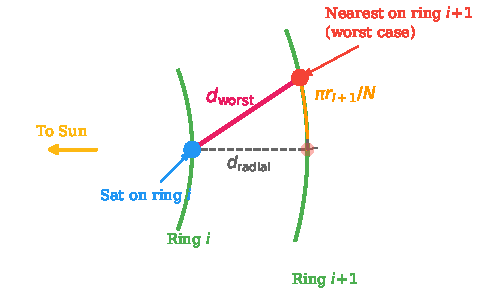
\includegraphics[width=0.55\columnwidth]{figures/bottleneck-geometry.pdf}
  \caption{Worst-case link geometry between adjacent rings. The link distance
    $d_{\mathrm{worst}}$ is the hypotenuse of the radial gap
    $d_{\mathrm{radial}}$ and the angular half-gap $\pi r_{i+1}/N$.}
  \label{fig:bottleneck-geometry}
\end{figure}

and the total constellation throughput, summed over all $N$ parallel routes, is
%
\begin{equation}\label{eq:T-total}
  T(N, R) \;=\; N \cdot C_{\text{route}}
  \;=\; \frac{N \, K}{\left(\dfrac{\Dem}{R+1}\right)^{\!2}
  + \left(\dfrac{\pi\,\rM}{N}\right)^{\!2}}
\end{equation}


\subsection{Optimal Distribution: Ring Count vs.\ Route Count}
\label{sec:optimal}

% TODO: Write prose explaining the tradeoff intuition before the derivation.
% Key idea: adding a ring reduces d_radial (inverse-square benefit is massive),
% but at fixed S it also reduces N = S/R, increasing the angular offset.
% The cubic R^3 term in the denominator means the angular penalty fights back
% harder than the 1/R radial benefit, but the inverse-square effect dominates
% until the crossover point.

For a fixed total satellite count $S = N R$, we substitute $N = S/R$ into
\cref{eq:T-total}. Approximating $R + 1 \approx R$ for large $R$:
%
\begin{equation}\label{eq:T-of-S-R}
  T(S, R) \;=\; \frac{S \, K}{\dfrac{\Dem^2}{R}
  \;+\; \dfrac{\pi^2 \rM^2 \, R^3}{S^2}}
\end{equation}
%
Maximising $T$ is equivalent to minimising the denominator
%
\begin{equation}
  g(R) \;=\; \frac{\Dem^2}{R} + \frac{\pi^2 \rM^2 \, R^3}{S^2}
\end{equation}
%
Setting $g'(R) = 0$:
%
\begin{align}
  g'(R) &= -\frac{\Dem^2}{R^2} + \frac{3\,\pi^2 \rM^2 \, R^2}{S^2} = 0
  \notag \\[6pt]
  R^4 &= \frac{\Dem^2 \, S^2}{3\,\pi^2\,\rM^2}
  \notag \\[6pt]
  \Ropt &= \sqrt{\frac{\Dem \cdot S}{\sqrt{3}\;\pi\;\rM}}
  \label{eq:R-opt}
\end{align}
%
or, in words:
%
\begin{quote}
\emph{The optimal number of relay rings equals the square root of the
Earth--Mars distance times the total satellite count, divided by
$\sqrt{3}\,\pi$ times Mars' orbital radius.}
\end{quote}
%
Numerically, with $\Dem = 78\;\text{Mkm}$ (average) and $\rM = 228\;\text{Mkm}$:
%
\begin{equation}
  \Ropt \approx 0.00251 \,\sqrt{S}
\end{equation}
%
The key implication: $\Ropt$ grows as $\sqrt{S}$. Doubling the total constellation
means $\approx 1.4\times$ more rings and $\approx 1.4\times$ more routes per ring.

\begin{figure}[t]
  \centering
  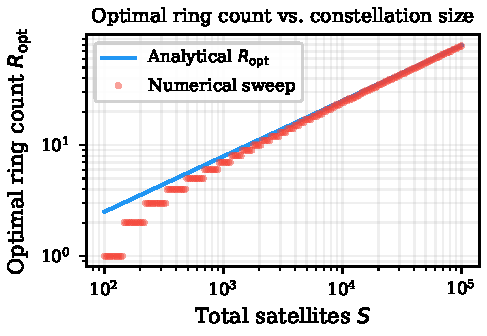
\includegraphics[width=0.65\columnwidth]{figures/optimal-R-vs-S.pdf}
  \caption{Optimal ring count $\Ropt$ as a function of total constellation size~$S$.
    The analytical prediction (\cref{eq:R-opt}) closely tracks the numerical sweep
    for $S > 1{,}000$.}
  \label{fig:optimal-R-vs-S}
\end{figure}


\subsection{Throughput Scaling Law}
\label{sec:scaling-law}

Substituting $\Ropt$ back into \cref{eq:T-of-S-R} yields the throughput as a function
of total satellite count alone. From $\Ropt^2 = \Dem S / (\sqrt{3}\,\pi\,\rM)$, we
compute each term of $g(\Ropt)$:
%
\begin{align}
  \frac{\Dem^2}{\Ropt}
  &= \Dem^{3/2}\,3^{1/4}\,(\pi\,\rM)^{1/2}\;S^{-1/2}
  \\[4pt]
  \frac{\pi^2 \rM^2 \, \Ropt^3}{S^2}
  &= \frac{\Dem^{3/2}\,(\pi\,\rM)^{1/2}}{3^{3/4}}\;S^{-1/2}
\end{align}
%
Summing (and noting $3^{1/4} + 3^{-3/4} = 3^{1/4}(1 + \tfrac{1}{3})
= \tfrac{4}{3}\,3^{1/4}$):
%
\begin{equation}
  g(\Ropt) = \frac{4}{3}\;3^{1/4}\;\Dem^{3/2}\;(\pi\,\rM)^{1/2}\;S^{-1/2}
\end{equation}
%
Therefore
%
\begin{equation}\label{eq:T-opt}
  \boxed{\;T_{\text{opt}}(S) \;=\; \frac{S\,K}{g(\Ropt)}
  \;=\; \frac{3^{3/4}\,K}{4\;\Dem^{3/2}\;\sqrt{\pi\,\rM}}
  \;\cdot\; S^{3/2}\;}
\end{equation}
%
The exponent $\tfrac{3}{2}$ is the central result: \textbf{throughput scales
super-linearly with satellite count.} Doubling the constellation increases throughput
by a factor of $2\sqrt{2} \approx 2.83$.

This super-linear scaling arises from two effects compounding. Adding satellites
simultaneously (i)~reduces inter-ring distances, improving per-link capacity
\emph{quadratically} via the inverse-square law, and (ii)~increases the number of
parallel routes, improving aggregate capacity \emph{linearly}.

\Cref{fig:throughput-vs-S} plots the throughput scaling on log--log axes, confirming
the $\tfrac{3}{2}$ slope across three orders of magnitude in~$S$.

\begin{figure}[t]
  \centering
  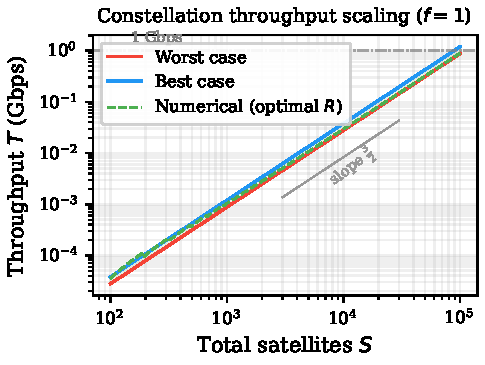
\includegraphics[width=0.65\columnwidth]{figures/throughput-vs-S.pdf}
  \caption{Constellation throughput vs.\ total satellite count ($f = 1$). The
    shaded region spans the best-case (radially aligned) and worst-case
    (half-arc offset) bounds, both scaling as $S^{3/2}$. The dashed line is
    the numerical optimum at integer~$R$. The horizontal line marks the
    1~Gbps target.}
  \label{fig:throughput-vs-S}
\end{figure}


\subsection{Best Case vs.\ Worst Case}
\label{sec:best-worst}

% TODO: Write prose contrasting the two bounds.

The derivation above uses the worst-case angular offset (half the arc spacing on the
outermost ring). In the best case---satellites on adjacent rings are radially aligned---the
angular offset vanishes and the link distance is purely radial:
%
\begin{equation}
  T_{\text{best}}(S) \;=\; \frac{K\,\sqrt{\alpha}}{\Dem^2} \; S^{3/2}
  \qquad\text{where}\quad \alpha = \frac{\Dem}{2\pi\,\rbar}
\end{equation}
%
with $\rbar = (\rE + \rM)/2$. Both bounds scale as $S^{3/2}$ and differ by a factor
of approximately~2. The analytical prediction matches numerical optimisation to within
2\% for $S > 50{,}000$ and within 10\% for $S > 5{,}000$.


\subsection{Equalized Ring Spacing}
\label{sec:equalized}

The uniform-spacing analysis of \cref{sec:optimal} places relay rings at equal radial
intervals $\Dem/(R+1)$. However, ring circumference grows with heliocentric
radius, so the angular half-gap $\pi r_i / N$ is largest on the outermost ring.
The bottleneck is therefore always the last hop---ring~$R$ to Mars---while inner
hops operate well below their capacity. This asymmetry suggests a refinement:
space the rings so that every inter-ring gap has the \emph{same} worst-case link
distance.

Let $d_{\mathrm{eq}}$ denote the common equalized link distance. For each gap $i$
between ring~$i$ and ring~$i\!+\!1$ (or Mars, for the last gap), the radial
spacing must satisfy
%
\begin{equation}\label{eq:d-eq-constraint}
  d_{\mathrm{radial},i} \;=\; \sqrt{d_{\mathrm{eq}}^2
  - \left(\frac{\pi\,r_{i+1}}{N}\right)^{\!2}}
\end{equation}
%
subject to the constraint that all radial gaps sum to $\Dem$:
%
\begin{equation}\label{eq:sum-constraint}
  \sum_{i=0}^{R} d_{\mathrm{radial},i} \;=\; \Dem
\end{equation}
%
Because $r_{i+1}$ increases outward, \cref{eq:d-eq-constraint} requires the radial
gap to \emph{shrink} with each successive ring: rings are packed more densely near
Mars, where the larger circumference would otherwise create a wider angular gap.
Near Earth, rings are spaced farther apart, since the smaller circumference leaves
room for larger radial hops without increasing the worst-case link distance.

No closed-form solution exists for $d_{\mathrm{eq}}$ because the ring positions
depend recursively on one another (each $r_{i+1}$ depends on the cumulative sum of
all preceding radial gaps). A simple binary search on $d_{\mathrm{eq}}$ converges
rapidly: build rings outward from Earth using \cref{eq:d-eq-constraint}, and adjust
$d_{\mathrm{eq}}$ until the final ring reaches Mars.

\begin{figure}[t]
  \centering
  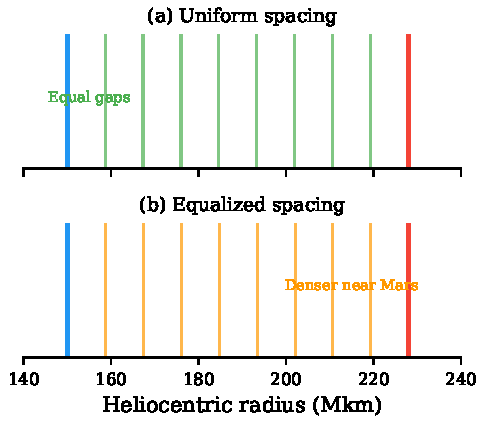
\includegraphics[width=0.65\columnwidth]{figures/equalized-spacing.pdf}
  \caption{Ring positions for $R = 8$ rings with $N = 500$ satellites per ring.
    \textbf{(a)}~Uniform spacing places rings at equal radial intervals.
    \textbf{(b)}~Equalized spacing packs rings more densely near Mars, where
    the larger circumference would otherwise create a wider angular gap.}
  \label{fig:equalized-spacing}
\end{figure}

The throughput improvement from equalized spacing is modest but consistent.
At the optimal ring count $\Ropt$ and for constellation sizes $S > 5{,}000$,
equalization yields approximately 8--9\% higher throughput than uniform spacing.
The improvement is smaller for low~$S$ (where few rings leave little room for
redistribution) and saturates for very large~$S$ (where $\Ropt$ is large enough
that radial gaps dominate the angular term everywhere). Crucially, the $S^{3/2}$
scaling exponent of \cref{eq:T-opt} is unchanged---equalized spacing modifies only
the prefactor.


\subsection{Effect of Orbital Eccentricity}
\label{sec:eccentricity}

The preceding analysis assumes circular orbits at mean radii. Mars' orbital
eccentricity $e_M = 0.0934$ causes its heliocentric distance to vary between
$\rM(1-e_M) \approx 207\;\text{Mkm}$ at periapsis and
$\rM(1+e_M) \approx 249\;\text{Mkm}$ at apoapsis, a ratio of
$(1+e_M)/(1-e_M) \approx 1.21$. Earth's eccentricity ($e_E \approx 0.017$) is
small enough to be negligible in comparison. This section shows that eccentricity
is a net positive for constellation throughput.

\subsubsection{Conformal Eccentric Rings}

A natural design response is to place relay satellites on \emph{conformal eccentric
orbits}: ring~$i$ has its semi-major axis and eccentricity interpolated between
Earth and Mars,
%
\begin{equation}
  a_i = \rE + \frac{i}{R+1}(\rM - \rE), \qquad
  e_i = e_E + \frac{i}{R+1}(e_M - e_E)
\end{equation}
%
with all orbits sharing the same argument of perihelion. At any true anomaly
$\theta$, ring~$i$ sits at heliocentric radius
%
\begin{equation}
  r_i(\theta) = \frac{a_i\,(1 - e_i^2)}{1 + e_i\cos\theta}
\end{equation}
%
This ensures that the relay chain tracks the time-varying Earth--Mars geometry:
when Mars is at periapsis, all rings are compressed inward; at apoapsis, they
expand outward.

\subsubsection{Jensen's Inequality Argument}

The throughput of a single route scales as $C \propto 1/d^2$, where $d$ is the
bottleneck link distance. Since $1/d^2$ is a \emph{convex} function of~$d$,
Jensen's inequality guarantees
%
\begin{equation}
  \bigl\langle 1/d^2 \bigr\rangle \;>\; 1/\langle d \rangle^2
\end{equation}
%
for any non-degenerate distribution of~$d$. Therefore the orbit-averaged
throughput of the eccentric constellation always exceeds the throughput of a
circular constellation evaluated at the mean distance. Eccentricity cannot hurt.

For a Keplerian orbit, the angle-averaged value of $(1 + e\cos\theta)^2$ is
exactly $1 + e^2/2$. Applied to Mars' eccentricity, this gives a pure convexity
gain factor of
%
\begin{equation}
  \bigl\langle (1 + e_M \cos\theta)^2 \bigr\rangle
  = 1 + \tfrac{1}{2}\,e_M^2 \approx 1.0044
\end{equation}
%
which is only 0.44\%---seemingly negligible.

\subsubsection{The Actual Gain Is Larger}

The full throughput gain exceeds the pure Jensen prediction because eccentricity
improves both terms in the bottleneck distance simultaneously. At Mars periapsis
($\theta = 0$), the Earth--Mars gap shrinks from the mean $\Dem \approx 78\;\text{Mkm}$
to approximately $59\;\text{Mkm}$, and the inverse-square law amplifies this
compression: capacity scales as $1/d^2$, so a 24\% reduction in distance yields a
73\% increase in per-link capacity. At the same time, Mars' orbital radius is
smaller at periapsis, which \emph{also} reduces the angular half-gap $\pi \rM / N$
on the outermost ring. Both terms in $d_{\max}^2 = d_{\mathrm{radial}}^2 +
(\pi \rM / N)^2$ shrink together.

At apoapsis ($\theta = \pi$), the situation reverses: the gap widens to
$\sim\!99\;\text{Mkm}$ and the angular offset grows. Routes through the apoapsis
side deliver only $\sim\!0.59\times$ the circular-case throughput. However, the
convexity of $1/d^2$ ensures that periapsis gains more than compensate apoapsis
losses.

Numerical evaluation over the full orbit yields an orbit-averaged throughput gain
of approximately 13--14\% relative to the circular baseline, consistent across
constellation sizes from $S = 1{,}000$ to $S = 50{,}000$. The crossover angle---where
eccentric throughput equals the circular value---occurs near $\theta \approx 85^\circ$.

\Cref{fig:eccentricity-profile} shows the angular throughput profile for
$S = 10{,}000$.

\begin{figure}[t]
  \centering
  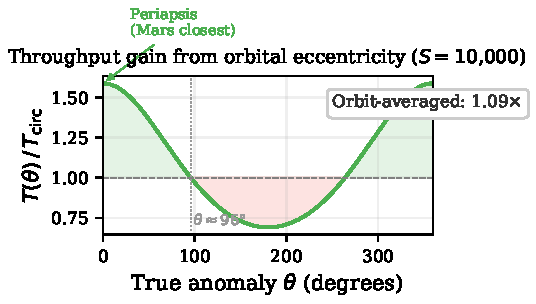
\includegraphics[width=0.65\columnwidth]{figures/eccentricity-profile.pdf}
  \caption{Throughput of the conformal eccentric constellation relative to the
    circular baseline, as a function of true anomaly~$\theta$.
    Green shading indicates where eccentricity helps; red where it hurts.
    The orbit-averaged gain is approximately 9\%, with the crossover near
    $\theta \approx 90^\circ$.}
  \label{fig:eccentricity-profile}
\end{figure}

As with equalized spacing, the $S^{3/2}$ scaling exponent is preserved.
Eccentricity modifies only the prefactor~$c$ in $T_{\mathrm{opt}} = c \cdot S^{3/2}$.
The two refinements---equalized spacing and eccentric conformality---are
complementary and can be applied jointly for a combined improvement of
approximately 20--25\% over the uniform circular baseline.


\subsection{Solar Exclusion Geometry}
\label{sec:solar-blinding}

Each relay satellite carries two laser terminals: one pointing radially inward
(Terminal~A) and one pointing radially outward (Terminal~B). Terminal~A receives
photons arriving from the next ring closer to the Sun. When the Sun, the
transmitting satellite, and the receiving satellite are nearly collinear, the
Sun's disk falls within or near the receiver's field of view, and the resulting
background noise overwhelms the signal. This \emph{solar blinding} constraint
imposes a minimum angular separation---the \emph{solar exclusion angle}
$\alpha_{\mathrm{exc}}$---between the Sun's \emph{limb} and the receiver
boresight. Measuring from the limb rather than the Sun centre makes the
constraint independent of heliocentric distance (the Sun's angular radius
$\rho_\odot = R_\odot / r$ ranges from $0.27^\circ$ at Earth to $0.18^\circ$
at Mars, but is already absorbed into the limb-referenced definition).
Typical values for free-space optical terminals range from
$3^\circ$ to $10^\circ$ from the limb~\cite{illuma-t2024}.

The problem is directional. For Earth-to-Mars data flow, the inward-pointing
Terminal~A on an outer-ring satellite receives from a transmitter that is closer
to the Sun; looking inward means looking roughly Sunward. For Mars-to-Earth flow,
Terminal~A receives from the \emph{outer} ring's transmitter, looking outward and
therefore away from the Sun. Solar blinding thus affects only half of the
bidirectional link: the Earth-to-Mars direction. The Mars-to-Earth direction is
geometrically immune.

\subsubsection{Natural Offset from Orbital Inclination}

Earth's orbital plane (the ecliptic) is inclined $1.85^\circ$ relative to Mars'
orbital plane. In the parallel constellation, each relay ring's orbital plane is
interpolated between the two: ring~$i$ has inclination
%
\begin{equation}
  \iota_i \;=\; \frac{i}{R+1}\;\iota_M
\end{equation}
%
where $\iota_M = 1.85^\circ$ is the Mars--ecliptic mutual inclination.
All rings share the same line of nodes (the intersection of the ecliptic and Mars'
orbital plane), with longitude of ascending node~$\Omega$.

At orbital longitude $\lambda$, the out-of-plane displacement of ring~$i$ relative
to the ecliptic is $z_i(\lambda) = r_i \sin\iota_i \sin(\lambda - \Omega)$.
Two adjacent rings ($i$ and $i\!+\!1$) therefore have an out-of-plane separation
%
\begin{equation}
  \Delta z_{i,i+1}(\lambda) \;\approx\;
  r_i \,\frac{\iota_M}{R+1}\;\sin(\lambda - \Omega)
\end{equation}
%
for small inclinations. The angular offset between the Sun direction (approximately
radially inward from any relay satellite) and the line connecting the satellite to
its inner-ring neighbour is
%
\begin{equation}\label{eq:alpha-offset}
  \alpha(\lambda) \;\approx\; \frac{\Delta z_{i,i+1}}{d_{\mathrm{radial}}}
  \;=\; \frac{r_i\,\iota_M}{(R+1)\,d_{\mathrm{radial}}}\;\sin(\lambda - \Omega)
\end{equation}
%
Since $d_{\mathrm{radial}} = \Dem/(R+1)$ and $r_i$ is of order $\rbar = (\rE + \rM)/2$,
the maximum angular offset from the Sun \emph{centre} simplifies to
%
\begin{equation}
  \alpha_{\mathrm{centre}} \;\approx\; \frac{\rbar\,\iota_M}{\Dem}
  \;\approx\; \frac{189 \times 0.0323}{78}
  \;\approx\; 0.078\;\text{rad}
  \;\approx\; 4.5^\circ
\end{equation}
%
Converting to a limb-referenced offset by subtracting the Sun's angular radius
$\rho_\odot = R_\odot / r \approx 0.22^\circ$ at the mean relay distance
$\rbar \approx 189\;\text{Mkm}$:
%
\begin{equation}\label{eq:alpha-max}
  \alpha_{\max} \;\approx\; \alpha_{\mathrm{centre}} - \rho_\odot
  \;\approx\; 4.5^\circ - 0.2^\circ
  \;\approx\; 4.3^\circ
\end{equation}
%
Both $\Delta z$ and $d_{\mathrm{radial}}$ scale as $1/(R+1)$, so their ratio
cancels the ring count: $\alpha_{\max}$ is independent of~$R$. The offset depends
only on the mean orbital radius, the inclination difference, the Earth--Mars gap,
and the solar angular radius.

\subsubsection{Blinding Zone Fraction}

Solar blinding occurs wherever $|\alpha(\lambda)| < \alpha_{\mathrm{exc}}$,
i.e.\ near the nodes where $\sin(\lambda - \Omega) \approx 0$.
The half-width of the blinding zone in orbital longitude is
%
\begin{equation}\label{eq:lambda-blind}
  \Delta\lambda_{\mathrm{blind}} \;=\; \arcsin\!\left(
  \frac{\alpha_{\mathrm{exc}}}{\alpha_{\max}}\right)
\end{equation}
%
Two nodes exist per orbit ($\lambda = \Omega$ and $\lambda = \Omega + 180^\circ$),
each contributing $2\Delta\lambda_{\mathrm{blind}}$ of affected arc, so the total
blinding fraction is
%
\begin{equation}\label{eq:f-blind}
  f_{\mathrm{blind}} \;=\; \frac{2}{\pi}\;\arcsin\!\left(
  \frac{\alpha_{\mathrm{exc}}}{\alpha_{\max}}\right)
\end{equation}
%
For $\alpha_{\mathrm{exc}} = 3^\circ$ and $\alpha_{\max} = 4.3^\circ$:
$f_{\mathrm{blind}} \approx 0.50$, meaning 50\% of the orbit is affected.
For $\alpha_{\mathrm{exc}} = 1.5^\circ$: $f_{\mathrm{blind}} \approx 0.23$.
For $\alpha_{\mathrm{exc}} = 4.3^\circ$ (matching $\alpha_{\max}$ exactly):
$f_{\mathrm{blind}} = 1$, and no orbital longitude is safe.

\Cref{fig:solar-blinding} shows the angular offset profile and blinding zone
for several exclusion angles.

\subsubsection{Mitigation: Lateral Targeting}

In the blinding zones near the nodes, a satellite on ring~$i\!+\!1$ cannot receive
from the radially nearest satellite on ring~$i$ because the Sun is too close to the
line of sight. Instead, it must target a \emph{laterally offset} neighbour---a
satellite on ring~$i$ that is displaced along the ring circumference by enough arc
to move the Sun out of the receiver's field of view.

The required lateral offset $\ell$ satisfies
$\alpha_{\mathrm{exc}} \approx \ell / d_{\mathrm{radial}}$, giving
%
\begin{equation}
  \ell \;\approx\; \alpha_{\mathrm{exc}} \cdot d_{\mathrm{radial}}
  \;=\; \frac{\alpha_{\mathrm{exc}} \cdot \Dem}{R+1}
\end{equation}
%
and the link distance increases from $d_{\mathrm{radial}}$ to
%
\begin{equation}\label{eq:d-blinding}
  d_{\mathrm{blind}} \;=\; \sqrt{d_{\mathrm{radial}}^2 + \ell^2}
  \;=\; d_{\mathrm{radial}}\,\sqrt{1 + \alpha_{\mathrm{exc}}^2}
\end{equation}
%
For $\alpha_{\mathrm{exc}} = 3^\circ \approx 0.052\;\text{rad}$, this gives
$d_{\mathrm{blind}} \approx 1.0014\,d_{\mathrm{radial}}$---a negligible 0.14\%
increase. Even at $\alpha_{\mathrm{exc}} = 10^\circ \approx 0.175\;\text{rad}$,
the penalty is only $\sqrt{1 + 0.0306} \approx 1.5\%$.

However, \cref{eq:d-blinding} assumes that a suitable laterally offset satellite
exists within the required angular displacement. The arc spacing between satellites
on ring~$i$ is $2\pi r_i / N$. If $\ell < 2\pi r_i / N$ (i.e.\ the offset fits
within one satellite spacing), the nearest non-blinded neighbour is the adjacent
satellite in the ring. If $\ell > 2\pi r_i / N$, multiple satellite spacings must
be skipped. In practice, for the constellation sizes considered here
($S > 5{,}000$), the arc spacing is much larger than the required offset $\ell$,
so the penalty is dominated by the worst-case angular half-gap $\pi r_i / N$
already accounted for in \cref{eq:d-worst}. The additional lateral displacement
from solar avoidance is a small perturbation on an already larger angular term.

The net effect on constellation throughput is modest. In the unaffected 52--78\%
of the orbit (depending on $\alpha_{\mathrm{exc}}$), throughput is unchanged.
In the blinding zones, the Earth-to-Mars direction suffers a per-link penalty of
at most a few percent, while the Mars-to-Earth direction is unaffected. The
orbit-averaged throughput reduction for the Earth-to-Mars direction is bounded by
%
\begin{equation}\label{eq:T-blind-penalty}
  \frac{\Delta T}{T} \;\lesssim\; f_{\mathrm{blind}} \cdot
  \frac{2\,\alpha_{\mathrm{exc}}^2}{1 + \alpha_{\mathrm{exc}}^2}
  \;\approx\; f_{\mathrm{blind}} \cdot 2\alpha_{\mathrm{exc}}^2
\end{equation}
%
For $\alpha_{\mathrm{exc}} = 3^\circ$: $\Delta T / T \lesssim 0.50 \times 0.005
\approx 0.3\%$. The solar exclusion constraint is a design consideration for
pointing control but does not materially affect the throughput scaling law.

\begin{figure}[t]
  \centering
  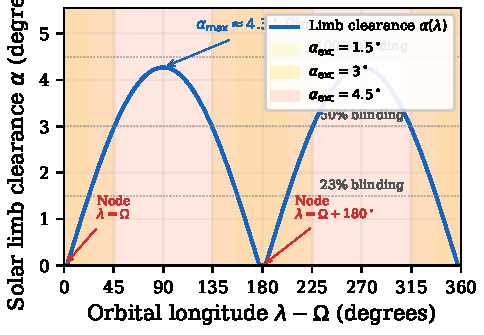
\includegraphics[width=0.75\columnwidth]{figures/solar-blinding.pdf}
  \caption{Solar limb clearance $\alpha(\lambda)$ between the Sun's limb and
    the inter-ring line of sight, as a function of orbital longitude~$\lambda$.
    The clearance peaks at $\alpha_{\max} \approx 4.3^\circ$ midway between nodes
    and vanishes at the nodes ($\lambda = \Omega, \Omega + 180^\circ$).
    Shaded regions show the blinding zones for exclusion angles of
    $1.5^\circ$, $3^\circ$, and $4.5^\circ$.}
  \label{fig:solar-blinding}
\end{figure}


\subsection{Cost--Throughput Trade-offs}
\label{sec:cost}

\Cref{fig:cost-per-mbps} shows the cost per Mbps as a function of ring count for
several constellation sizes, using the following cost model: \$5M per satellite
(production), \$0.2M per laser terminal (two per satellite), and \$20M per
Starship launch carrying 20~satellites. The total cost is
$S \times 5.4\text{M} + \lceil S/20 \rceil \times 20\text{M}$.

For every constellation size, cost efficiency improves dramatically as rings are
added---moving from 1~ring to the optimal ring count reduces cost per Mbps by
over an order of magnitude. The optimal ring count closely tracks the analytical
$\Ropt$ from \cref{eq:R-opt}. Beyond the optimum, adding more rings (at fixed~$S$)
reduces $N$ and therefore the number of parallel routes, causing the angular offset
to dominate and throughput to fall.

\begin{figure}[t]
  \centering
  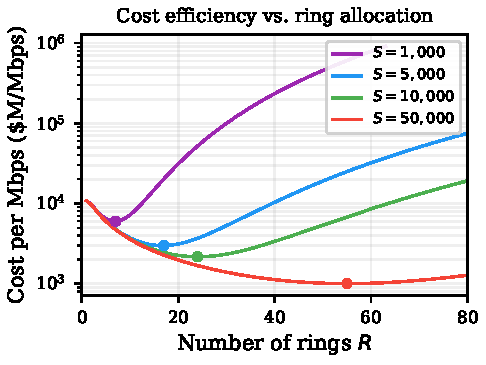
\includegraphics[width=0.65\columnwidth]{figures/cost-per-mbps.pdf}
  \caption{Cost per Mbps vs.\ ring count for several constellation sizes.
    Dots mark the optimal ring allocation for each~$S$.
    Cost model: \$5.4M/satellite (production + 2 terminals),
    \$20M/Starship launch (20~satellites per launch).}
  \label{fig:cost-per-mbps}
\end{figure}